	% Chapter Template

\chapter{Methodology} % Main chapter title

\label{Chapter3} % Change X to a consecutive number; for referencing this chapter elsewhere, use \ref{ChapterX}

\lhead{Chapter 3. \emph{Methodology}} % Change X to a consecutive number; this is for the header on each page - perhaps a shortened title

On an abstract level, the model consists of an environment comprising of numerous agents, and a few companies. This thesis specifically focuses on the various strategies used by the companies to attract the agents, and try to measure its efficiency in terms of the related costs and benefits. Based on these measurements, a company could determine the optimal strategy to maximize its efficiency for the targeted section or sub-subsection of agents.

%----------------------------------------------------------------------------------------
%	SECTION 1
%----------------------------------------------------------------------------------------

\section{The Companies}

The companies only exist in a superficial form in the model. In this model, each company plays its role by providing a central point for the agents to cluster about, and the movement of this point itself denotes effort made by the company, which in turn incurs a cost to the company.

The author decided to keep this model limited to two companies competing for the same spot, i.e., any agent cannot totally belong to both companies at the same time. 
The primary reasons for this were limitations of time and computation power, in that order.


%-----------------------------------
%	SECTION 2
%-----------------------------------
\section{The Agents}

The agents in this model are simpler constructs, each  having a ``color" attribute, and this attribute changes as the agents tend to believe in either of the companies.

Structurally, each agent has the following attributes :

\begin{enumerate}
\item Id
\item x-position coordinate
\item y-position coordinate
\item Colour value
\item Influence value
\end{enumerate}

During its lifetime, an agent has constant value for its Id, but the rest of its attributes may change. The influence value of the agent is determined as a function of the number of connections it makes, and remains constant once the whole network is created. All other attributes, however, may change throughout the simulation.

%-----------------------------------
%	SECTION 3
%-----------------------------------

\section{Connections}
The connections between the agents form in such a manner that the model satisfies the requirements of free-scaling. The implementation is based on algorithm ~\ref{alg1}, which is a modified form of the B-A algorithm.

\subsection{The World}
The model is first built based on two fixed parameters, and then the simulation runs on it.
The author starts building the model for a fixed number of total agents \emph{N}, and predefined average connectivity \emph{d} in the environment.
The initialization of the model begins with the creation of a small, fully connected network, and then, with time, new agents are added to this network, and these agents form the connections following the rules of preferential attachment.
The exact method of forming a connection was modified by the author, so as to further trick the environment. This allowed simulation of scenarios where it is possible to form a number of connections, but only a fraction of those connections are actually formed. This was achieved by employing a `weight' modifier on the probability of an agent to form a connection. This weight, in turn, is defined for every possible pair of agents, and is based on the difference in the value of a special attribute ``like-mindedness", defined for each agent in a uniform, pseudo-random manner.
This attribute is not considered an essential attribute because it may or may not be used, in various simulations. However, as an effect of using this modifier, the number of connections for an agent comes down considerably, while the nature of the connections still remain same, and the network remains scale free.


\begin{figure}
\begin{center}
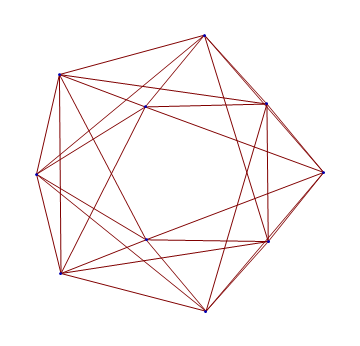
\includegraphics[scale=0.75]{Figures/network_init}
\end{center}
\caption{Sample of Initial network with 10 nodes}
\label{fig:network_init}
\end{figure}

\begin{figure}
\begin{center}
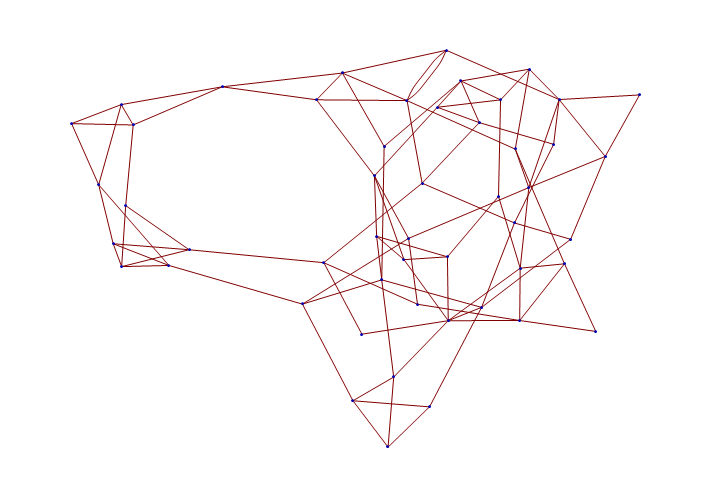
\includegraphics[scale=0.5]{Figures/network_final}
\end{center}
\caption{Sample of Final network with 50 nodes}
\label{fig:network_final}
\end{figure}

The concept of starting with a smaller network and growing it is explained in detail in Chapter~\ref{Chapter2} in section~\ref{sec:model} and examples are shown in figures~\ref{fig:network_init} and ~\ref{fig:network_final}.

\subsection{The Simulation} 
 
The simulation begins with allocating ``influence" value to each existing agent, as a function of the number of connections it has in the network. This makes sure that the most-connected agents get a chance to be more influential. 
After this, values are uniformly assigned to all agents for the ``color" attribute, and then they are seeded to belong to different companies. 20 \% was the value chosen by the author for initial amount of seeding, for the following combination of reasons:

\begin{enumerate}
\item It allows for equal amount of seeding in both companies.
\item It allows for double amount of seeding in a neutral company.
\item After above mentioned allocations, it leaves equal amount of distribution randomly, to simulate chance.
\end{enumerate}

The above rules give us the formula

\begin{eqnarray}
company_1 + company_2 + company_{neutral} + company_{random} = 100 \nonumber \\
\Rightarrow x + x + 2x + x = 100 \% \nonumber \\
\Rightarrow x = 20 \% 
\label{eqn:seed fraction}
\end{eqnarray}

Then, the simulation is run, where in each time step, an edge is selected randomly, and an exchange could happen if the \textit{FromNode} of this edge belongs to one of the two companies. Here, ``belonging to company" refers to the value of the ``color" attribute for the agent.
After this, the influence value of the \textit{FromNode} is subjected to a randomly selected threshold, and upon satisfaction, the actual communication occurs. The threshold is lowered depending on a company's efforts towards attracting the customer. 

The selection of the edge depicts existence of a connection, while satisfaction of the threshold depicts the actual communication. This constraint was included to make the simulation model even closer to real-life. 
Hence, a higher effort would result in more cost, but would give a company higher chances of a successful communication.

For every successful communication, the agents shift their ``color" attribute a fraction towards the influencing company. This shift also translates to their x-y coordinate, which is shown in the presentation. The important aspect here is that these changes in color and x-y coordinates, while not always causally related, are always correlated. 

For the companies, however, it has different significance. Whenever an agent has moved closer, the companies also make an effort and move some fraction towards the agents. The amount of distance moved by the company represents the effort it makes, and is determined by the company policy. These movements also incurs the cost to the company, and a combined function of the gain and this cost determines the effectiveness of the policy.

Towards the end of the campaigning, a company may increase their effort to maximise chances of gain. This is achieved in the model by doubling the shift amount whenever a certain amount has been spent on the campaigning.


In the end, the gain and cost are calculated for the companies using the equation~\ref{eqn:cost_gain}. Since cost is already lesser than the gain, this function was kept linear.

\begin{eqnarray}
function = gain - cost \\
\label{eqn:cost_gain}
\end{eqnarray}

%----------------------------------------------------------------------------------------
%	SECTION 4
%----------------------------------------------------------------------------------------


\section{Definitions}
\label{sec:definitions}
\begin{enumerate}
\item \emph{Fully Connected}

It follows the standard definition that each node is connected to every other node. The initial network is formed in such a manner that it is fully connected and satisfies the average number of total connections.

\item \emph{Like-mindedness}

It is a special attribute of the agents, that is used in this model to modify the probability of formation of a new connection between two agents. It simulates the real life phenomenon that people with similar interests may be more likely to form a connection. 

This subject is very vast in itself, and covers a wide ground ~\cite{jung1921question, Wilt08extraversion}. This is also helpful in showing the aspect that some people may be introverts or extroverts. However, that aspect is not simulated in detail in this model.

\item \emph{Weight}

The \textit{weight} is the difference in \textit{like-mindedness} of two agents. It is calculated as 

\begin{eqnarray}
weight_{j,k} = abs( likemindedness_{j} - likemindedness_{k} )
\label{eqn:weight}
\end{eqnarray}

\item \emph{Company Centre}

The company is not implemented as a structural entity, rather, the company centre is used to keep track of the attitude of the agents towards the company, and also to track the effort and cost on the part of the company.

\item \emph{Influence}

This attribute determines the chances of an agent to influence another agent. As in real life, we allow more connected agents a chance to be more influential, but ultimately, there is no deterministic end to the model, and whether or not an actual communication takes place and an agent gets influenced is always determined by a randomly determined threshold. 
This is calculated as a function, described by equation ~\ref{eqn:influence}, of the number of connections the agent makes.

\begin{eqnarray}
influence_{i} = \frac{connections_i}{connections_{max}} 
\label{eqn:influence} 
\end{eqnarray}

\item \emph{Shift}

This shift represents a change in the state of the overall system. For an agent, a shift in its color attribute represents the agent leaning towards a company. This shift is correlated with the same ratio of change in the agent's x-y coordinate, used for visualization purposes.
For a company, the shift only occurs in its x-y coordinate, which is caused by the x-y shift of the agent, and this change represents two things : 
\subitem[a] The speed and frequency of movement represent the effort taken by the company
\subitem[b] The distance moved represent the cost incurred to the company
\end{enumerate}

\clearpage
%----------------------------------------------------------------------------------------
%	SECTION 5
%----------------------------------------------------------------------------------------

\section{Algorithms}

\begin{algorithm}
\caption{Create Scale-Free Network}
\label{alg1}
\begin{algorithmic}
\STATE N : Input, total number of agents
\STATE D : Input, average number of connections
\IF {$D < N+1$}
	\STATE Form a \emph{fully connected} network with D+1 agents
\ENDIF 
\STATE implement $CG$
\STATE $i \gets D+1$
\WHILE{$i < N$} 
	\STATE $Agent_i \gets newAgent$
	\STATE assign $likemindedness$ 
	\STATE implement $PA$
	\STATE $k \gets 0$
	\WHILE{$k \leq \frac{D}{2}$}
		\STATE calculate $probability_{basic}$ based on equation~\ref{eqn:PA}
		\STATE compute $weight$ based on equation~\ref{eqn:weight} 
		\STATE $probability_{attachment} \gets  probability_{basic} + weight$ 
		\STATE $Agent_i$ forms $connection_k$ , based on $probability_{attachment}$
	\ENDWHILE	
\ENDWHILE
\end{algorithmic}
\end{algorithm}

\clearpage

\begin{algorithm}
\caption{Simulation}
\label{alg2}
\begin{algorithmic}
\STATE assign $centres_{company}$
\STATE assign $effort_{company}$
\STATE calculate $influence$ based on equation~\ref{eqn:influence}
\STATE assign \emph{color} to all agents
\STATE seed $20\% $ agents to $color1$
\STATE seed $20\%$ agents to $color50$
\STATE seed $40\%$ agents to $color25$
\STATE seed $2 \emph{most influential}$ agents to different companies
\STATE $J$ : number of iterations
\STATE $i \gets 0$
\WHILE{$i \leq J$}
	\STATE select $edge_i$
	\IF{ $FromNode_{color}$ = $\emph{color1}$ OR $\emph{color50}$ }
		\STATE select $threshold$
		\STATE $threshold$ = $threshold$ - $effort_{company}$
		\IF{ $ FromNode_{influence} \geq threshold $ }
			\STATE $ToNode_{color} \gets ToNode_{color} + \emph{shift}$
			\STATE $ToNode_{x-coordinate} \gets ToNode_{x-coordinate} + \emph{shift}$
			\STATE $ToNode_{y-coordinate} \gets ToNode_{y-coordinate} + \emph{shift}$
			\STATE $Company_{x-coordinate} \gets Company_{x-coordinate} + \emph{shift}$
			\STATE $Company_{y-coordinate} \gets Company_{y-coordinate} + \emph{shift}$
		\ENDIF
	\ENDIF
\ENDWHILE
\end{algorithmic}
\end{algorithm}

\clearpage